\chapter{Related Work}\label{cha:related}
Object detection using CNNs is a fairly new area of study, and as such, its application in the domain of pollen counting is lacking in literature.
Examining related work therefore requires a wider field of view and must explore the ways in which similar methods have been used to solve similar problems.
This chapter is broken into two main sections.
Section~\ref{sec:rel-cnn} will examine the various object detection frameworks and their use within microscopy.
Section~\ref{sec:rel-pollen} will detail the various methods that have been employed in relation to the specific domain of automated pollen counting.

\section{Convolutional Neural Networks}\label{sec:rel-cnn}
Before CNNs, the task of classifying images was usually highly dependent on the problem domain.
Careful feature engineering was used to extract a set of parameters which were then classified using a statistical model.
A CNN fundamentally changes this landscape by removing all manual feature engineering.
Over the last 10 years, CNNs have risen to prominence as the state of the art in image processing.
Raw images are classified directly, with little consideration of the specific domain.
The trade-off is the near insatiable thirst these models have for labelled training data required to train them.

\subsection{Object detection}
With the quality of image classifiers rising, focus has been given to the more complex task of object detection, where the model must identify the location of objects within an image, as well as their class.
Work on this problem was kickstarted by\ \textcite{girshick_rich_2014} with the proposed method: \textit{Regions with CNN features} (R-CNN), a three stage system which first identifies `regions of interests' within an image, before classifying them using a CNN and statistical classifier.
They later proposed Fast R-CNN and Faster R-CNN which improved the learning and inference time, as well as the robustness, of the original model.

R-CNN has three main modules.
First, bounding boxes are proposed using selective search, an algorithm where different similarity measures are first used to segment the image into a myriad of small sections, before these are then selectively grouped together into larger \textit{regions of interest}.
Each region is then resized and fed into a CNN, the second stage, which produces a feature embedding which is finally classified using an SVM, the third stage.
A major computational bottleneck was having to process each region proposal independently through the second and third stage.

Fast R-CNN removes the second and third stages and replaces them with a new CNN which takes as input the whole image and the region proposals and generated predictions for all regions in one go.
This new second stage also predicts offsets for the proposed boxes, allowing it to refine the proposals from the first stage.

Faster R-CNN replaces the first stage with a Region Proposal Network (RPN), a fully convolutional deep neural network which produces a fixed number of bounding boxes together with an `objectness' score for each box.
The RPN introduces the concept of anchors, which are points in the image used to regress bounding boxes.
After a set of convolutional layers, a \(n\by n\) feature map is outputted.
Imagining a set of anchor boxes imposed upon the image which are centered on each cell of the feature map, the dimensions of regions of interest are computed by producing regressions of the anchor boxes by running a convolution over the feature map with a small kernel.
At each step of the convolution, one parameter of a anchor box centered at the middle of the receptive field is produced.
With 4 filters, the center point, height and width of an anchor box can be regressed to a region of interest in proximity to the anchor.
Using a RPN allows of training of both stages of the detector, significantly increasing the performance.
Following the release of Faster R-CNN, the amount of research attempting to automate various object detection tasks has increased.

In many domains there is usually a positive correlation between the cost of data and its quality.
Often times methods that are proposed therefore become prohibitively expensive because they make use of higher quality data only available to the researchers.
CNN based methods have however shown that high quality models can be created using lower quality data.\ \textcite{el_melegy_automatic_2019} gave a good example of this.
A Faster R-CNN method is proposed for detecting tuberculosis bacilli in LM slides.
The model they propose is able to outperform all previous traditional models, many of which use higher quality imaging methods.
The type of images the model uses are very difficult to diagnose manually but are by far the most available in the field.
The model also solves an issue present in most of the previous work, namely, how to actually automate the process of diagnosis.
Previous work is based on pre-segmented images which are then classified, which requires a human expert.
This is common for a lot of research where a problem involves localization.

\subsection{Single stage detectors}\label{sec:ssd}
Common to the R-CNN family of methods is the use of two separate stages, one for identifying regions of interest in an image, and one for classifying objects in those regions.
This adds considerable complexity in that both systems require separate training and hyper-parameter tuning.
These methods have been successfully utilized in many domains, including the only published attempt at pollen grain detection by\ \cite{gallardo_caballero_precise_2019}.
The inference speed is however prohibitively slow for tasks that require real-time performance.
Overall, there is an obvious trend in the evolution of the two stage systems where stages are replaced by a CNN\@.
This trend continues to its logical conclusion with the development of the single stage detector (SSD).

\begin{figure}[htbp]
    \centering
    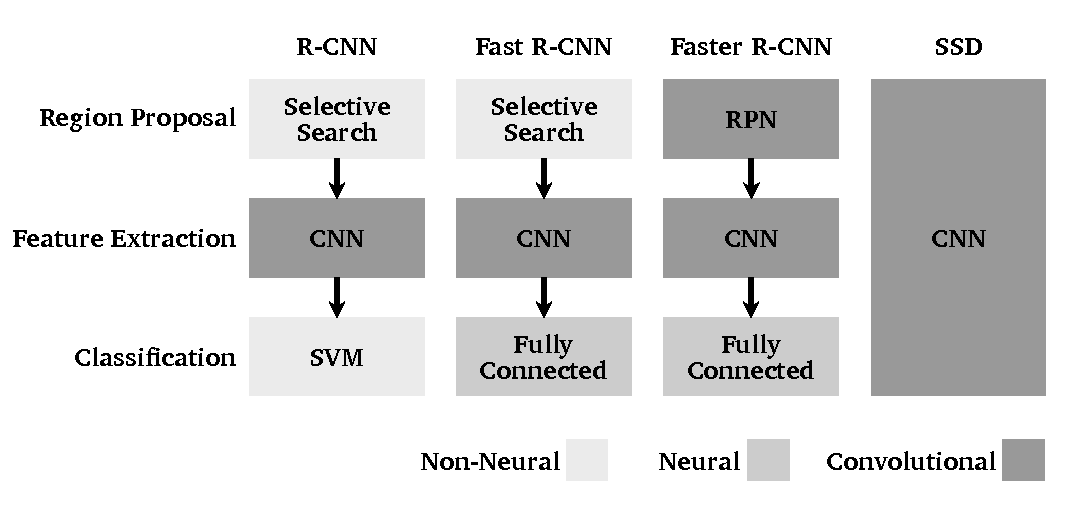
\includegraphics[width=0.75\textwidth]{figs/related/detector_evolution.pdf}
    \caption[Evolution of object detection models]{Object detection models show a gradual shift towards all tasks being performed by a CNN}\label{fig:related-detectors}
  \end{figure}

This class of model comprises only a single CNN, responsible for both localizing and classifying objects.
These models can be trained in one pass, and feature inference speeds orders of magnitude faster than Faster R-CNN\@.
One of the first methods was the Single Shot Multibox Detector (SSD), proposed by\ \textcite{liu_ssd_2016}, which is the model implemented in Section~\ref{sec:method-arch}.
It was one of the first systems to demonstrate that a single fully convolutional model could vastly improve inference speeds without compromising accuracy.

The architecture resembles the RPN from Faster R-CNN\@.
Like an RPN, SSD predicts bounding box offsets for a fixed number of \textit{default bounding boxes}.
Boxes with a predefined aspect ratio and size are centered on each cell of a feature map and a small-kerneled convolution predicts regression parameters for the position and size of these boxes.
A separate, but identically configured, convolutional layer produces class confidence scores for each default box.
The output of the network is thus both regression parameters and class confidence scores for a fixed number of default bounding boxes.

SSD makes predictions from multiple feature layers, and the default boxes are scaled up as the depth of the feature map in the network increases.
This allows the network to predict objects at different scales in the image.
The training objective for SSD is created by matching default boxes with overlapping ground truth boxes based on their IoU score.
This match is then used to produce a target for the regression parameters and class for every positively matched default box.
The model is trained by a linear combination of two separate loss functions, one for the bounding box regressions, and one for the class confidences.
Most default boxes are not matched to any ground truth box which causes an imbalance in the loss function.
To balance out the ratio of negative and positive examples in the training objective, only the negative examples with the highest loss values are included in the final loss calculation.

As of writing, there are no published attempts of using a single stage detector to count pollen grains, but there are examples of its use in similar domains.\ \cite{liu_brain_2018} uses an SSD model to detect brain slices used in an automatic sample preparation system.
The model was chosen for its speed and accuracy, both important in real-time detection.
The model was also simplified because the range of scales to be detected was narrower than what the standard SSD model has implemented.
This simplification could also prove relevant to a pollen detection task where grains are similar in both size and shape.
Because of the structure of the SSD model, this simplification is achieved just by removing layers from the model, thus removing predictions from those scales.
Results show that the simplified model increased both accuracy and speed over the original.

You Only Look Once (YOLO) is a very popular single stage model, its release closely following SSD\ \parencite{redmon2016look}.
As with R-CNN it has been released in many versions with iterative improvements.
It is similar to SSD in that it also predicts box offsets and class scores for a fixed number of bounding boxes.
Specifically, YOLO divides an input image into a grid and then predicts box offsets for a fixed number of bounding boxes centered in each grid square (but not regressed from default boxes), and class confidences for each grid square (not each bounding box).
Both SSD and YOLO also use transfer learning in the form of an initial feature extractor which is transferred from a pertained classification model.
The later versions of YOLO also feature multiple extraction layers which improve predictions for smaller objects, which was one of the major weaknesses of the initial version.

Recently, multiple papers using YOLO models have been published showing promising results in areas similar to pollen counting.\ \textcite{chibuta_real_time_2020} used a modified version of the third iteration of YOLO to screen blood smears for malaria.
Diagnosing malaria is very costly because it requires manual analysis of blood samples.
Similar to Tuberculosis, the areas with the highest prevalence of the disease, are those where the primary screening technique uses light field microscopy.
The presented model uses a smaller feature extractor and fewer extraction layers to optimize for speed on basic hardware.
The model has \( \simeq 99\% \) fewer parameters than the standard YOLOv3 implementation and still performs at the same level as both human experts, and its unoptimized equivalent.

Another area of study of relevance to this thesis is blood cell counting.
A complete blood count is a test that is often requested when evaluating general health and involves a manual count of blood cells within a sample.
The current standard process requires human expert analysis and is prone to error.\ \textcite{islam_machine_2019} proposed a YOLO model which accurately localizes and classifies blood cells using standard LM images of a blood smear.
The YOLO model has not been modified apart from changing the number of classes to 3 (Red, White, and Platelets).
They do however change the inference routine to optimize the count for each of the three cell types.
As with the aforementioned RPN, YOLO predicts an objectness score for each bounding box, and normally considers a box to be a positive match if the score exceeds a threshold.\ \citeauthor{islam_machine_2019} show that, rather than using only one threshold value for all classes, a higher overall accuracy can be reached by filtering boxes for each class independently with different thresholds.
This points towards a larger issue of choosing both the algorithms that are used to filter the predictions made by these models and their hyper parameters.
The difference between how many raw predictions a model makes, and the number of objects an image contains is usually many orders of magnitude.
The method used to filter the predictions is therefore crucial to the performance of the model, and also highly dependent on the domain.

\section{Automated Pollen Detection}\label{sec:rel-pollen}
There have been many attempts at pollen grain classification over the last three decades.
These have been nicely summarized by\ \textcite{sevillano_improving_2018}.
Most are statistical classifiers using selected features from pollen images.
The earlier attempts can be grouped into three categories.
The first focuses on morphological features such as shape, size and symmetry.
The second type uses the texture of the grain surface as the discriminating feature.
The last group uses a hybrid approach which combines morphological and texture features.
These methods have been able to successfully classify pollen to a degree comparable to human experts, but all rely on careful feature engineering.
Of the earlier methods, the most successful utilize images taken through SEM, which is a much more expensive imaging technique than standard LM imaging.

\subsection{Classical methods}
As a precursor to the newer systems, it is pertinent to cover the earlier attempts at solving the problem of automated pollen counting.
The first attempt, by\ \textcite{langford_computerized_1990}, used grey scale SEM images of the surface texture on pollen grains.
16 feature measures, based on a Grey-tone spatial dependence analysis, were then produced and classified using Linear Discriminant Analysis (LDA).
This technique was successful, but required manual analysis for each class, making it difficult to apply to new datasets or other taxa of pollen.

Other attempts were made over the next decade, some using morphological features instead of surface texture, but they follow the same basic procedure of feature engineering followed by a statistical classifier.
The next major contribution was made in\ \textcite{li_pollen_1999}, in which very high accuracy was achieved using LM images.
The major disadvantage of LM imaging was the shallow depth of field causing only portions of the pollen grains to be in focus.
This reduction of image quality caused a loss in accuracy of the LDA based methods.
The new method exchanged the classifier with a Multi-Layer Perceptron and achieved higher scores than previous methods using a simpler set of feature measures.
The main limitation was the lack of processing power at the time which meant that the method could not scale to larger sets of images.

As computational power rose, there were also attempts made at localizing grains.\ \cite{france_new_2000} presented a hybrid solution featuring both classical and neural methods.
The localization is handled by a K-means classifier coupled with a shape and size filter, producing segments of the image likely to contain pollen.
A trained classifier is then used to classify the grains.
The results were promising, but the system was also very limited.
Firstly, it was very sensitive to focus, and could only work with grains perfectly within the depth of field.
Secondly the segmentation algorithm only worked on sparse images with a certain amount space between grains.
These same issues also create problems for modern systems, albeit not to the same extent.

Convolution has been an important tool in image processing since before CNNs gained traction.
Using hand crafted filters, many basic features such as edges, can be extracted from an image.
This technique was employed by\ \textcite{DaoodICPR16b} with good results.
The system used a SVM for the final classification, but demonstrated the viability of using convolutional filters as feature extractors.
This system in some ways bridges the gap towards the CNN models, but crucially lacks the ability the learn which features should be extracted.
This is the fundamental deficiency common to all the classical methods: they rely on human expert knowledge to adapt each method for use in the specific domain.

\subsection{CNN methods}
CNNs have all but taken over as the standard in image classification, and this is also the case in pollen detection.
Recently all the proposed methods involve a deep convolutional neural network as the main feature extractor.
Comparing the different models that have been presented is however very challenging.
Most use self-collected datasets which vary in size, both with respect to the number of classes and examples per class.
There is also an inherent difference in the difficulty of separating instances within any given dataset because some types of pollen are much more similar than others.
Meaningful comparisons are therefore difficult to make.
A performance comparison is however not strictly relevant to this thesis, seeing as they are all classifiers, which cannot be used to locate pollen grains.

{\cite{daood_pollen_2016}} presented a CNN method that was used on both a LM and SEM dataset and compared the results with many of the classic statistical methods, showing the clear benefit of using a CNN model.
A second network was also implemented which used transfer learning to further improve accuracy.
Data augmentation was used to combat the small size of the dataset, something that has been a pervading issue for most of the presented solutions.
The paper showed that, although a higher accuracy was obtained on the SEM data, the models were fully capable of achieving good results using LM images.
Both transfer learning and data augmentation is featured in most of the subsequently published papers.

{\cite{sevillano_improving_2018}} later gave more evidence for the supremacy of CNN methods by applying three different convolutional models on a publicly available dataset {POLENE23E}, which at that point only had been classified using classic methods.
All three models used a CNN as the feature extractor and they all performed well, doubling the precision over the state of the art.
The results also show that there are only insignificant improvements when using a linear discriminant classifier on top of the CNN\@.

Common to all the mentioned methods is that the data they rely on is LM images of a single grain.
This ignores two important factors, firstly and most obvious is the fact that none of these models can be used directly to count pollen grains, only to classify pre-segmented images of singular grains.
This also leads into the second important factor of dealing with LM images of pollen grains at different focal planes.

Grains of pollen on a slide are not distributed across one focal plane and are not oriented in the same direction.
Grains are scattered across all three axes and because of the narrow depth of field of the microscope are only partially visible when focused on.
The depth of field is in fact so shallow that only parts of the surface ornamentation appear clear.
For a human operator this is not a problem as the focus can be adjusted to reveal the entire grain in turn, with static images however, dealing with this lack of complete information is an open question.

For the models we have covered, this means that they potentially are missing out on features because they only rely on an image of a single focal plane.
In the case of classification, one possible remedy for this is to use a stack of images, named a \textit{z-stack}, taken at different focal planes and process the stack as one unit.\ \textcite{DaoodAndRibeiro_2018} uses this approach.
The model they propose takes as input a sequence of 10 images taken of pollen grains spanning the whole grain, and classifies it using a network which combines a \textit{recurrent} neural network (RNN) and a convolutional neural network.
A recurrent neural network is a special type of network used to process sequences of information, e.g.\ signals, text, and in this case, 3D image stacks.
The RNN has a memory unit which `remembers' the past elements of a sequence and uses this to process sequential data.
The model first uses the CNN to create a feature embedding for each frame independently, the sequence is then classified by an RNN\@.
The result is a reportedly 100\% accurate model over a dataset with 10 classes.

The main conclusion drawn is that the z-stack benefits from being processed as a sequence, and not as independent samples, but the results show only small improvements from using the RNN over a majority-vote system using classifications from the CNN directly.
There is also no clear strategy for extending the system for grain detection, which limits its utility.

The last model we will look at is also the only published work attempting to use a CNN to localize pollen grains in slide images.\ \textcite{gallardo_caballero_precise_2019} uses Faster R-CNN to detect pollen grains of various types within unaltered LM images of pollen grains.
The model does not perform classification of the grains it localizes.
They report very high values for both precision and recall but use a slightly modified definition of IoU when calculating these values.
Multifocal data is used only when running inference by combining the detections from the entire z-stack as one single prediction.

The dataset they use was created by filming the slide whilst moving the focus plane across the pollen grains.
Based on an auto-focused keyframe, 10 frames were extracted before and after the keyframe, creating a 21-frame z-stack.
From this, two datasets where created.
In the first one, the pollen grains were labeled in the frame where they appeared sharpest and ignored in all other images.
In the second dataset, the grains were labeled in all images throughout the sequence.

The performance of the model was calculated by stacking the individual predictions from all focal planes together, and then performing a standard filtering algorithm.
The reported results are very good, but it is probable that the results are inflated due to the elimination of class predictions from the problem.
The definition of IoU is also changed so that comparison to other object detection models is impossible.
The effect this has on the values for recall and precision is not declared.

Two trials were run to compare the performance obtained from the two datasets, and values for recall and precision were high for both (above .98), with the non-blurred trial having slightly higher precision.
The authors conclude that there do not seem to be any real differences in performance between models trained with or without blurred images, but their method of using detections from multiple focal planes in each prediction hides the effects that blur has on the model hard to pin-point.

How to utilize the information contained in a z-stack is a very open question.
Both methods presented above using z-stacks achieved good results, but neither attempts to explain how the models are affected by the different sharpness valued in the data.
Rather, they aggregate information from all images, which hides how the model responds to each static image.
Gathering data on how sharpness affects the model could provide valuable insight into this relationship.

In this section we have detailed both how CNNs are used to solve object detection problems, and how the field of automated pollen grain analysis has evolved from using highly specialized hand-crafted feature extractors, to being dominated by generalized CNN based frameworks.
Of most significance to this research are the modifications that have been successfully made to CNN models used in similar fields to pollen grain counting, as well as the different techniques that have been used to make use of multifocal data.
